\documentclass[11pt]{article}

\usepackage[utf8]{inputenc}
\usepackage[T1]{fontenc}

\usepackage[a4paper, left=2cm, right=2cm, top=3.5cm, bottom=3.5cm]{geometry}
\usepackage[french]{babel}

% Paragraph spacing
\setlength{\parskip}{1em}

% Fancy headers
\usepackage{fancyhdr}

% Captions for subfigures
\usepackage{subcaption}


% Code highlighting
\usepackage{minted}

% Footnote inside a caption
\usepackage{fnpos}
\usepackage{ftnxtra}

% Colored text, provides \textcolor{color}{text}
\usepackage{xcolor}

% Maths
\usepackage{amsmath}
\usepackage{amssymb}

% Todo notes
\usepackage{todonotes}

% Table of contents for bibliography
\usepackage[nottoc]{tocbibind}

% Inline monospace font
\def\code#1{\texttt{#1}}

% Figures
\usepackage{graphicx}

% Draw figures
\usepackage{tikz}

% Code listing
\usepackage{listings}

% Tikz node rotation
\usetikzlibrary{positioning}

% Turing machine
\usetikzlibrary{chains,fit,shapes}

% Usage: \rotnode[options]{rotation}{text}
\newcommand\rotnode[3][]{%
\node [#1, opacity=0.0] (tmp) {#3};
\node [draw, rotate around={#2:(tmp.center)}] at (tmp) {#3};
}

% remove extra space
\newcommand{\squeezeup}{\vspace{-4.5cm}}

% Clickable links
\usepackage{hyperref}
% Table of contents depth
\setcounter{tocdepth}{2}

% Inline code
\usepackage{listings}
\usepackage{color}

\title{Systèmes d'exploitation - Moniteurs II}

\author{Othmane AJDOR}
\date{2018-2019}

\begin{document}
\maketitle

\pagebreak
\tableofcontents
\pagebreak

\section{But}
\begin{itemize}
	\item Synchronisation de threads, 1 même programme , mémoire partagée
	\item Ensemble de fonctions en exclusion mutuelle (pas de problème de concurrence)
\end{itemize}
Le problème est de prendre des decisions alors qu'on est en exclusion mutuelle.
On empeche le programme d'évoluer (mise en attente à l'aide de variables de condition), ainsi, on relache l'exclusion mutuelle et les threads sont placés dans une file d'attente.

\section{Barrière à N}
On veut que N threads appellent barriereN()
\begin{figure}[h!]
	\centering
	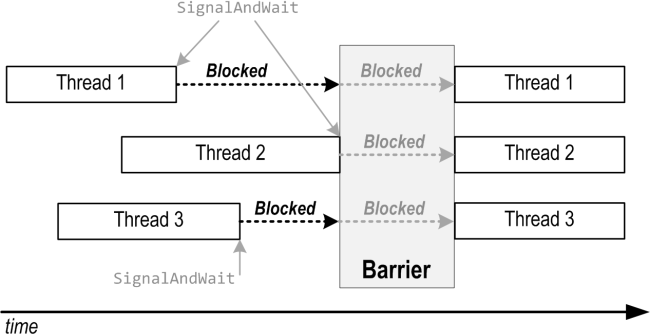
\includegraphics[scale=2]{img/barrier.png}
\end{figure}

On utilise un mutex[lock|unlock], la fonction cnd\_t[wait|signal].\\
cnd\_signal(\&c) réveille un thread.

\begin{minted}[frame=single]{c}
	int compteur = 0;
	const N = 42;
	mtx_t m;
	cnd_t c;
	barriereN(){
		mtx_lock();
		compteur++;
		while(compteur < N){
			cnd_wait(&c, &m);
		}
		// reveil en cascade, le N+1 reveil le premier et ainsi de suite
		cnd_signal(&c); 
		mtx_unlock();
	}
\end{minted}

\section{Allocateur}
On se contente de reveiller tous les threads en attente.\\
cnd\_broadcast(\&c) reveille tous les threads.
\vspace{-0.4cm}
\begin{minted}[frame=single]{c}
	const int resource = N;
	mtx_t m;
	cnd_t c;
	allocation(int n){
		mtx_lock(&m);
		while(resource<n){
			cnd_wait(&c, &m);
		}
		resource -= n;
		mtx_unlock(&m);
	}

	liberation(int n){
		mtx_lock(&m);
		resource += n;
		cnd_broadcast(&c);
		mtx_unlock(&m);
	}
\end{minted}

\textbf{\textcolor{red}{CODE CI-DESSOUS FAUX}}\\
Dans le cas où deux threads arrivent, ils se reveillent et s'endorment entre eux avec le code suivant:
\vspace{-0.4cm}
\begin{minted}[frame=single]{c}
	const int resource = N;
	mtx_t m;
	cnd_t c;
	allocation(int n){
		mtx_lock(&m);
		while(resource<n){
			cnd_wait(&c, &m);
			cnd_signal(&c);
		}
		resource -= n;
		mtx_unlock(&m);
	}

	liberation(int n){
		mtx_lock(&m);
		resource += n;
		cnd_signal(&c);
		mtx_unlock(&m);
	}
\end{minted}

\pagebreak

\section{Producteurs Consommateurs}

\begin{figure}[h!]
	\centering
	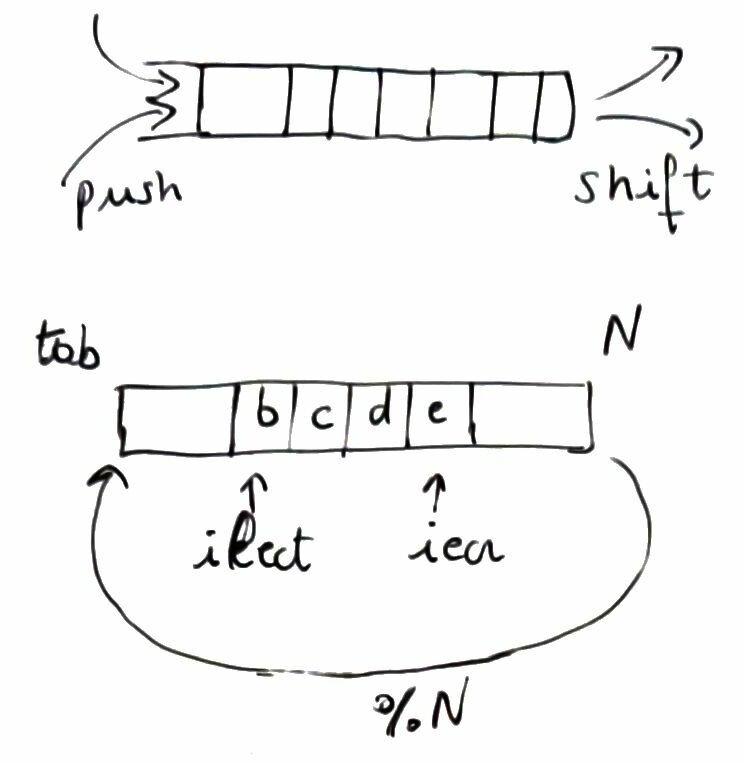
\includegraphics[scale=0.3]{img/prod_cons.jpg}
\end{figure}

\begin{minted}[frame=single]{c}
	int iecr = 0; // indice d'ecriture
	int ilect = 0; // indice de lecture
	int nb = 0;
	mtx_t m;
	cnd_t fp; // file de producteurs
	cnd_t fc; // file de consomateurs
	Msg Tab[N];
	
	push(Msg msg){
		mtx_lock(&m);
		while (nb == N){
			cnd_wait(&fp, &m)
		}
		tab[iecr] = msg;
		nb++;
		iecr++;
		iecr %= N;
		cnd_signal(&fc)
		mtx_unlock(&m);
	}






	Msg shift(){
		mtx_lock(&m);
		while (nb == 0){
			cnd_wait(&c, &m);
		}
		Msg msg = tab[ilect];
		nb--;
		ilect++;
		ilect %= N;
		cnd_signal(&fp);	
		mtx_unlock(&m);
		return msg;
	}
\end{minted}
Les modifications des indices ilect et iecr doivent être faites au même endroit pour lire/ecrire dans la même case du tableau.

\pagebreak

\section{Lecteurs-Redacteurs (shared mutex)}
On dispose d'une base de données où on stock des informations, on autorise les lectures à plusieurs mais les ecritures seront limités à 1 thread à la fois et il sera \underline{tout seul} (pas de lecture, pas d'autres redacteurs).

On utilise un compteur de lecteurs et un compteurs de redacteurs.\\
Lorsqu'un redacteur finit d'ecrire, il faut donner la priorité aux redacteurs. L'inconvenient de cela est lorsqu'il y a beaucoup d'ecrivains, les lecteurs ne passent jamais. Cette priorité peut donc causer une famine de lecture. On peut aussi créer une famine d'écriture si la priorité aux lecteurs est choisie (pire qu'une famine de lecture).

Pour reveiller la bonne personne, on a besoin de compter les lecteurs et redacteurs en attente.

\begin{minted}[frame=single]{c}
	int nblect;
	bool ecr;
	int nblect_att;
	int nbecr_att;
	mtx_t m;
	cnd_t clect;
	cnd_t cecr;

	debut_lire(){
		mtx_lock(&m);
		while (nbecr_att > 0 || ecr){
			nblect_att++;
			cnd_wait(&clect, &m);
			nblect_att--;
		}
		nblect++;
		mtx_unlock(&m);
	}

	fin_lire(){
		mtx_lock(&m);
		if (nblect_att != 0 && nblect == 0){
			cnd_signal(&cecr);
		}
		mtx_unlock(&m);
	}

	debut_ecr(){
		mtx_lock(&m);
		while (ecr || nblect != 0){
			nbecr_att++;
			cnd_wait(&cecr, &m)
			nbecr_att--;
		}
		ecr = true;
		mtx_unlock(&m);
	}

	fin_ecr(){
		mtx_lock(&m);
		ecr = false;
		if (nbecr_att > 0){
			cnd_signal(&cecr);
		} else {
			if (nblect_att > 0){
				cnd_broadcast(&clect);
			}
		}
		mtx_unlock(&m);
	}
\end{minted}

Si on retire les compteurs des lecteurs et redacteurs en attente, le code devient:
\begin{minted}[frame=single]{c}
	int nblect;
	bool ecr;
	int nblect_att;
	int nbecr_att;
	mtx_t m;
	cnd_t clect;
	cnd_t cecr;

	debut_lire(){
		mtx_lock(&m);
		nblect++;
		while (ecr){
			cnd_wait(&clect, &m);
		}
		nblect++;
		mtx_unlock(&m);
	}

	fin_lire(){
		mtx_lock(&m);
		if (nblect == 0){
			cnd_signal(&cecr);
		}
		mtx_unlock(&m);
	}

	debut_ecr(){
		mtx_lock(&m);
		while (ecr || nblect != 0){
			cnd_wait(&cecr, &m)
		}
		ecr = true;
		mtx_unlock(&m);
	}

	fin_ecr(){
		mtx_lock(&m);
		ecr = false;
		if (nblect > 0){
			cnd_broadcast(&clect);
		} else {
			cnd_signal(&cecr);
		}
		mtx_unlock(&m);
	}
\end{minted}
\end{document}